\documentclass[12pt,a4paper]{article}

% ----------------------------------------------------------
% PAQUETES DE FORMATO GENERAL
% ----------------------------------------------------------
\usepackage[english]{babel}
\usepackage[utf8]{inputenc}
\usepackage[T1]{fontenc}
\usepackage{mathptmx}
\usepackage{geometry}
\usepackage{setspace}
\usepackage{graphicx}
\usepackage{booktabs}
\usepackage{array}
\usepackage{longtable}
\usepackage{float}
\usepackage{caption}
\usepackage{url}
\usepackage[hidelinks]{hyperref}
\usepackage{amsmath}
\usepackage{enumitem}
\usepackage{microtype}
\usepackage{xcolor}

\geometry{left=2.5cm,right=2.5cm,top=2.5cm,bottom=2.5cm}
\setstretch{1.15}
\graphicspath{{figures/}}
\Urlmuskip=0mu plus 1mu

\captionsetup{font=small,labelfont=bf,justification=centering}
\setlist[itemize]{leftmargin=1.2cm}
\setlist[enumerate]{leftmargin=1.2cm}

% ----------------------------------------------------------
% DATOS DEL ARTÍCULO
% ----------------------------------------------------------
\title{\textbf{Arquitectura Distribuida para el Análisis Predictivo de Farmacovigilancia sobre Reportes FAERS con Control de Fuga de Información}}

\author{Jaime Arriagada Rosas · Nicolás Barrientos Sabaleta · Gustavo Flores Lama ·\\
Nicolás Andrade Barrios · Sebastián Pinto Espinosa\\[0.3cm]
\small Facultad de Ingeniería, Universidad Andrés Bello, Santiago, Chile\\
\small Corresponding author: n.barrientossabaleta@uandresbello.edu}

\date{}

\begin{document}

\maketitle

\begin{abstract}
La farmacovigilancia moderna requiere analizar grandes volúmenes de reportes de eventos adversos para detectar señales de riesgo asociadas al uso de medicamentos. Este artículo presenta el diseño e implementación de una arquitectura distribuida para escalar el análisis predictivo de reportes del sistema \textit{FDA Adverse Event Reporting System} (FAERS). La propuesta procesa aproximadamente 385.288 casos únicos del cuarto trimestre de 2025, distribuidos en siete tablas relacionales: DEMO, DRUG, REAC, OUTC, INDI, THER y RPSR. La metodología integra limpieza automatizada, almacenamiento columnar en Parquet, análisis exploratorio de datos, procesamiento distribuido mediante \textit{Reduce-Side Join} con MapReduce, cálculo de señales estadísticas de seguridad mediante PRR y Chi-cuadrado con corrección de Yates, técnicas de balanceo de clases y una etapa de modelado predictivo de severidad clínica. A diferencia de versiones previas, este trabajo incorpora un control riguroso de fuga de información (\textit{data leakage}) en dos capas: (i) la partición \textit{train/test} se realiza antes de cualquier ajuste de codificadores o aplicación de SMOTE, manteniendo el conjunto de prueba completamente intacto; y (ii) se neutraliza el \textit{target leakage} en la variable de reacción adversa mediante un enmascaramiento por entropía de los términos MedDRA que actúan como \textit{proxies} del desenlace. Asimismo, el componente de modelado pasa de un clasificador único a una comparación sistemática de cuatro modelos (Regresión Logística, Random Forest, XGBoost y LightGBM) con validación cruzada estratificada de cinco pliegues y SMOTE encapsulado dentro del \textit{pipeline} de validación. Finalmente, se conserva un componente de streaming basado en Apache Kafka, con respaldo en cola local, para habilitar detección temprana de combinaciones fármaco--reacción críticas. Es importante precisar el alcance del aporte: el volumen de un único trimestre (5.473.692 registros, 385.288 casos únicos) es tratable en memoria con herramientas de un solo nodo, por lo que la contribución no reside en superar una restricción de cómputo actual, sino en proponer y validar una \textit{arquitectura preparada para escalar} cuya lógica de unión \textit{mapper--reducer} es portable, sin cambios sustanciales, hacia un clúster Hadoop real cuando se acumulen múltiples trimestres o se integren fuentes adicionales. Los resultados muestran que el flujo procesa 5.473.692 registros, consolida información clínica en un dataset analítico, mitiga el desbalance de severidad y produce métricas de evaluación honestas: el mejor modelo (Random Forest) alcanza una exactitud de 0,689 y un \(F_1\) macro de 0,517 sobre datos reales sin contaminación sintética. La arquitectura propuesta constituye una base reproducible y portable para análisis de farmacovigilancia a escala creciente.
\end{abstract}

\noindent\textbf{Keywords:} FAERS; farmacovigilancia; arquitectura distribuida; MapReduce; Hadoop; Kafka; Random Forest; XGBoost; LightGBM; data leakage; señales de seguridad; aprendizaje automático; PRR; Chi-cuadrado.

\section{Introduction}

Los sistemas de farmacovigilancia tienen como finalidad identificar, evaluar y prevenir riesgos asociados al uso de medicamentos después de su comercialización. En este contexto, el sistema FAERS de la FDA constituye una de las fuentes públicas más relevantes para el análisis de eventos adversos, ya que recopila reportes enviados por profesionales de la salud, pacientes y fabricantes. Sin embargo, la utilidad analítica de esta información depende directamente de la capacidad de procesar datos heterogéneos, voluminosos y distribuidos en múltiples tablas relacionales.

El problema central abordado en este trabajo consiste en determinar, a partir de reportes FAERS, qué medicamentos presentan mayor riesgo de causar eventos adversos, con una metodología estadísticamente interpretable, portable hacia infraestructura distribuida y, sobre todo, metodológicamente honesta. El enfoque tradicional basado en procesamiento puramente local resulta progresivamente insuficiente a medida que se acumulan trimestres y se busca unir cientos de millones de registros provenientes de tablas como DEMO, DRUG, REAC, OUTC, INDI, THER y RPSR. Estas tablas se relacionan mediante el identificador \texttt{primaryid}, pero presentan diferencias de formato, valores nulos, alta cardinalidad, duplicados y desbalance clínico.

Un riesgo frecuente y subestimado en modelos predictivos de severidad sobre datos clínicos es la fuga de información, que puede manifestarse de dos formas: cuando el preprocesamiento (codificación o sobremuestreo) se ajusta sobre el conjunto completo antes de particionar, y cuando una variable predictora codifica de forma casi determinista la etiqueta objetivo. En FAERS, dado que la severidad se deriva de la tabla OUTC, ciertos términos MedDRA (por ejemplo, \textit{Death} o \textit{Cardiac Arrest}) están tan concentrados en un único nivel de severidad que actúan como \textit{proxies} del desenlace y inflan artificialmente el desempeño. Este trabajo aborda explícitamente ambos problemas.

Frente a este escenario, se propone una arquitectura híbrida que combina procesamiento histórico por lotes (\textit{batch}) y detección temprana en tiempo real (\textit{streaming}). El componente batch utiliza Hadoop/MapReduce, implementado mediante \textit{mrjob}, para ejecutar un \textit{Reduce-Side Join} distribuido entre las siete tablas FAERS. Luego, el sistema calcula señales de seguridad mediante el \textit{Proportional Reporting Ratio} (PRR) y la prueba Chi-cuadrado con corrección de Yates. Paralelamente, se entrena y compara un conjunto de clasificadores multiclase para predecir el nivel de severidad clínica de nuevos eventos adversos en una escala ordinal de cinco niveles, bajo controles estrictos contra la fuga de información.

Este artículo contribuye con: (1) una arquitectura reproducible para procesar reportes FAERS mediante capas de almacenamiento y procesamiento distribuido; (2) un pipeline de limpieza y análisis exploratorio adaptado a tablas de farmacovigilancia; (3) un proceso de consolidación basado en \textit{Reduce-Side Join}; (4) un módulo de detección de señales estadísticas; (5) un protocolo de modelado predictivo de severidad con control de fuga de información en dos capas y comparación de cuatro algoritmos; y (6) un componente de streaming para evaluar nuevos reportes y generar alertas tempranas.

\section{Background and Related Work}

\subsection{Farmacovigilancia y reportes espontáneos}
FAERS es un sistema de reportes espontáneos utilizado para vigilancia poscomercialización. Su valor principal radica en permitir la identificación temprana de patrones inusuales entre medicamentos y eventos adversos. No obstante, debido a su naturaleza espontánea, los reportes no deben interpretarse como incidencia clínica directa. Las frecuencias observadas reflejan notificaciones, no necesariamente prevalencia real de eventos en la población expuesta.

En farmacovigilancia, las métricas de desproporcionalidad se utilizan para priorizar asociaciones fármaco--reacción que aparecen con frecuencia superior a la esperada. Entre las métricas más utilizadas se encuentran el PRR~\cite{evans2001}, el Reporting Odds Ratio (ROR), el Information Component (IC) bayesiano del BCPNN, el Empirical Bayes Geometric Mean (EBGM) del Multi-item Gamma Poisson Shrinker y la prueba Chi-cuadrado. Estudios comparativos sobre FAERS han evaluado la sensibilidad relativa de estos métodos usando controles positivos y negativos, encontrando concordancia razonable entre ellos pero sin una superioridad clara de los métodos frecuentistas sobre los bayesianos, y confirmando una fuerte dependencia de la sensibilidad respecto del número de reportes disponibles~\cite{disproportionalityAssessment2015}. En la práctica regulatoria y de investigación es habitual exigir la concordancia simultánea de varios criterios (por ejemplo, ROR, PRR, BCPNN y MGPS con sus respectivos umbrales) para declarar una señal robusta~\cite{ticagrelorFaers2024,il1faers2024}. En este proyecto se seleccionan PRR y Chi-cuadrado con corrección de Yates por su interpretabilidad, bajo costo computacional y uso histórico en sistemas regulatorios~\cite{ema2006}; reconocemos como limitación que el PRR es sensible a falsos positivos cuando el número de reportes es bajo, razón por la cual imponemos un soporte mínimo de tres reportes, criterio coherente con el umbral usado de forma generalizada en la literatura de señales.

Una consideración transversal en todos estos trabajos es que FAERS requiere una curación sustancial antes de su uso analítico: la deduplicación de versiones de un mismo caso, la normalización de nombres de fármacos a vocabularios estándar (RxNorm) y el mapeo de desenlaces a terminologías clínicas (SNOMED-CT) afectan materialmente los resultados, como evidencia el recurso estandarizado AEOLUS~\cite{banda2016}. Nuestro pipeline de limpieza por capas aborda una parte de estos problemas (deduplicación y normalización de \texttt{primaryid} y de tipos), aunque no realiza el mapeo completo a vocabularios estándar, lo que constituye una limitación reconocida frente a estos recursos curados.

\subsection{Big Data aplicado a datos clínicos y elección de motor}
El crecimiento sostenido de datos clínicos y farmacológicos ha impulsado el uso de herramientas Big Data para resolver problemas de volumen, velocidad y variedad. Hadoop y MapReduce permiten distribuir operaciones intensivas como agrupamientos, conteos y uniones por clave. En el caso de FAERS, el uso de \texttt{primaryid} como identificador común permite ejecutar uniones distribuidas entre tablas con millones de registros.

Es necesario, sin embargo, distinguir entre el volumen de un trimestre individual y el volumen agregado de la serie histórica. Un trimestre como el aquí analizado es perfectamente tratable con bibliotecas de un solo nodo (pandas, Polars o DuckDB), e incluso con un motor distribuido moderno como Apache Spark, que hoy supera a MapReduce clásico en rendimiento y ergonomía. Reconocemos abiertamente esta tensión: para el dato puntual, MapReduce constituye sobre-ingeniería. La justificación de nuestra elección no es de rendimiento sino de \textit{portabilidad de la lógica}: al expresar la unión como funciones \textit{mapper} y \textit{reducer} desacopladas del motor, la misma lógica se ejecuta localmente en desarrollo y migra a un clúster Hadoop o a Spark (vía su API equivalente) cuando el corpus longitudinal lo amerite, sin reescribir la regla de negocio. El formato Parquet complementa esta arquitectura al permitir almacenamiento columnar, compresión eficiente y lectura selectiva de columnas, característica útil en pipelines donde no todas las columnas son necesarias en cada etapa.

\subsection{Fuga de información en modelos clínicos}
La fuga de información ocurre cuando información que no estaría disponible en el momento de la predicción influye en el ajuste del modelo, produciendo estimaciones de desempeño optimistas e irreproducibles~\cite{kaufman2012}. Dos formas son particularmente relevantes en este dominio. La primera es la fuga de preprocesamiento, que aparece cuando codificadores, escaladores o técnicas de balanceo como SMOTE se ajustan sobre el conjunto completo antes de separar entrenamiento y prueba; la práctica correcta es particionar primero y ajustar cualquier transformación solo sobre el conjunto de entrenamiento. La segunda es la fuga de objetivo (\textit{target leakage}), que surge cuando una variable predictora determina casi por completo la etiqueta. Dado que en este trabajo la severidad se deriva determinísticamente de OUTC, los términos MedDRA fuertemente asociados a un único desenlace deben tratarse como \textit{proxies} del objetivo y no como predictores legítimos.

\subsection{Aprendizaje automático para predicción de severidad}
Los modelos de aprendizaje automático permiten complementar el análisis estadístico tradicional con capacidad predictiva. Existe un cuerpo creciente de literatura que aplica ML específicamente sobre FAERS para predecir severidad de eventos adversos. Trabajos recientes en oncología han entrenado modelos de \textit{gradient boosting} sobre millones de casos FAERS para predecir eventos adversos graves, reportando mejoras sustanciales sobre la regresión logística e identificando predictores clínicamente interpretables mediante análisis SHAP~\cite{oncoSAE2026}. De manera análoga, estudios sobre inhibidores de puntos de control inmunitario (PD-1/PD-L1) han comparado LightGBM y CatBoost frente a líneas base como Random Forest para clasificar severidad en esquemas binarios (grave vs. no grave), evaluando AUC, exactitud y \(F_1\) sobre conjuntos de prueba retenidos~\cite{pd1faers2025}. Otros trabajos abordan la automatización de la detección de eventos adversos sobre FAERS con diversos algoritmos, reportando que cerca de un tercio de los reportes corresponde a desenlaces graves~\cite{automatingADE2024}, y enfoques de ensamble combinan múltiples clasificadores (Random Forest, Gradient Boosting, XGBoost, redes neuronales y SVM) con puntuación ponderada por severidad para detección temprana de reacciones raras~\cite{ensembleRare2026}. Encuestas sistemáticas del área sintetizan las tareas, datos y métodos de ML usados en estudios de reacciones adversas~\cite{nguyenSurvey2021}.

Frente a este panorama, nuestro trabajo se diferencia en tres aspectos. Primero, la mayoría de los estudios citados restringen el análisis a una clase terapéutica específica (oncología, inmunoterapia) y a esquemas de severidad binarios, mientras que aquí se aborda el corpus completo de un trimestre con una escala ordinal de cinco niveles, problema multiclase más difícil. Segundo, y de forma central, gran parte de la literatura no audita explícitamente la fuga de objetivo derivada de que la severidad se computa a partir de los mismos desenlaces que coexisten con términos MedDRA fuertemente asociados; nuestro control de \textit{proxies} por entropía aborda directamente esa fuente de optimismo. Tercero, las métricas honestas aquí reportadas (Random Forest, exactitud 0,689, \(F_1\) macro 0,517 sobre cinco clases) son naturalmente más moderadas que los AUC altos de los esquemas binarios y específicos de fármaco, y por tanto no son directamente comparables: la diferencia de techo de desempeño es atribuible al mayor número de clases y a la neutralización deliberada de variables que codifican el desenlace.

Para datos tabulares con variables categóricas de alta cardinalidad, los ensambles de árboles como Random Forest, así como los algoritmos de \textit{gradient boosting} (XGBoost y LightGBM), son adecuados porque pueden modelar relaciones no lineales sin requerir escalamiento estricto de variables. La inclusión de una Regresión Logística como línea base permite contextualizar la ganancia real de los modelos más complejos. El uso de \texttt{class\_weight='balanced'} y de sobremuestreo sintético mediante SMOTE~\cite{chawla2002} ayuda a ajustar la influencia de clases minoritarias, aspecto relevante en problemas clínicos donde los eventos graves suelen ser menos frecuentes que los leves.

\subsection{Procesamiento en tiempo real}
Apache Kafka permite desacoplar productores y consumidores de eventos, habilitando arquitecturas de streaming. En farmacovigilancia, esta capacidad permite evaluar reportes nuevos sin esperar el cierre de un trimestre o la ejecución de un lote completo. Este trabajo integra Kafka como componente de detección temprana, permitiendo cruzar reportes entrantes contra señales históricas indexadas y contra el modelo predictivo previamente entrenado.

\section{Methodology}

\subsection{Data Source and Study Dataset}
El dataset utilizado corresponde a reportes FAERS del cuarto trimestre de 2025. Los archivos originales se encuentran en formato de texto plano, delimitados por el carácter \texttt{\$} y codificados en Latin-1. El sistema procesa siete tablas vinculadas por \texttt{primaryid}. La Tabla~\ref{tab:faers_tables} resume las tablas utilizadas, sus archivos, cantidad de registros y contenido principal.

\begin{table}[H]
\centering
\caption{Tablas originales de FAERS procesadas en el proyecto.}
\label{tab:faers_tables}
\small
\begin{tabular}{@{}llll@{}}
\toprule
\textbf{Tabla} & \textbf{Archivo} & \textbf{Registros} & \textbf{Descripción} \\
\midrule
DEMO & DEMO25Q4.txt & 385.288 & Datos demográficos. \\
DRUG & DRUG25Q4.txt & 1.815.349 & Medicamentos y dosis. \\
REAC & REAC25Q4.txt & 1.349.105 & Reacciones MedDRA PT. \\
OUTC & OUTC25Q4.txt & 289.721 & Desenlaces clínicos. \\
INDI & INDI25Q4.txt & 1.168.789 & Indicaciones. \\
THER & THER25Q4.txt & 454.746 & Terapias y duración. \\
RPSR & RPSR25Q4.txt & 10.694 & Fuente del reporte. \\
\bottomrule
\end{tabular}
\end{table}

El volumen total procesado corresponde a 5.473.692 registros distribuidos en las siete tablas, con 385.288 casos únicos identificados en DEMO. Conviene ser explícitos respecto del alcance: este volumen, para un único trimestre, cabe holgadamente en la memoria de una estación de trabajo y puede procesarse con herramientas de un solo nodo (pandas, Polars, DuckDB) o con un motor distribuido como Spark. Por tanto, la elección de MapReduce vía \textit{mrjob} no se justifica por una necesidad de cómputo del trimestre actual, sino como una decisión de diseño orientada a la \textit{portabilidad} y la \textit{escalabilidad incremental}: la lógica de unión expresada como \textit{mapper} y \textit{reducer} es agnóstica al motor y puede trasladarse, sin reescribir la lógica de negocio, a un clúster Hadoop real cuando el corpus crezca por la acumulación longitudinal de trimestres (FAERS publica cuatro por año, con un histórico de más de una década) o por la integración de fuentes externas como VigiBase u OpenFDA. Esta separación entre lógica de negocio e infraestructura de ejecución es precisamente la propiedad que se valida en este trabajo a escala de un trimestre, dejando la demostración empírica del escalamiento multitrimestral como trabajo futuro (Sección~\ref{sec:future}).

\subsection{Storage Architecture}
La arquitectura de almacenamiento sigue un patrón por capas: \texttt{raw}, \texttt{clean}, \texttt{staging}, \texttt{joined} y \texttt{balanced}. La capa \texttt{raw} conserva los archivos originales sin modificación. La capa \texttt{clean} almacena tablas limpias en formato Parquet con compresión Snappy. La capa \texttt{staging} contiene archivos JSONL etiquetados por tabla para ser procesados por MapReduce, así como los conjuntos de \textit{features} de entrenamiento y prueba ya particionados. La capa \texttt{joined} guarda el dataset consolidado resultante del \textit{Reduce-Side Join}. Finalmente, la capa \texttt{balanced} contiene versiones balanceadas del dataset para experimentación.

\subsection{Exploratory Data Analysis}
El análisis exploratorio se implementó mediante nueve scripts especializados ejecutados secuencialmente (\texttt{s01} a \texttt{s09}). Estos módulos generan resúmenes estadísticos, análisis de valores nulos, distribuciones de variables, conteos por tabla, detección de duplicados, análisis de reacciones, distribución de desenlaces clínicos, análisis temporal y matrices de co-ocurrencia fármaco--reacción.

\begin{figure}[H]
\centering
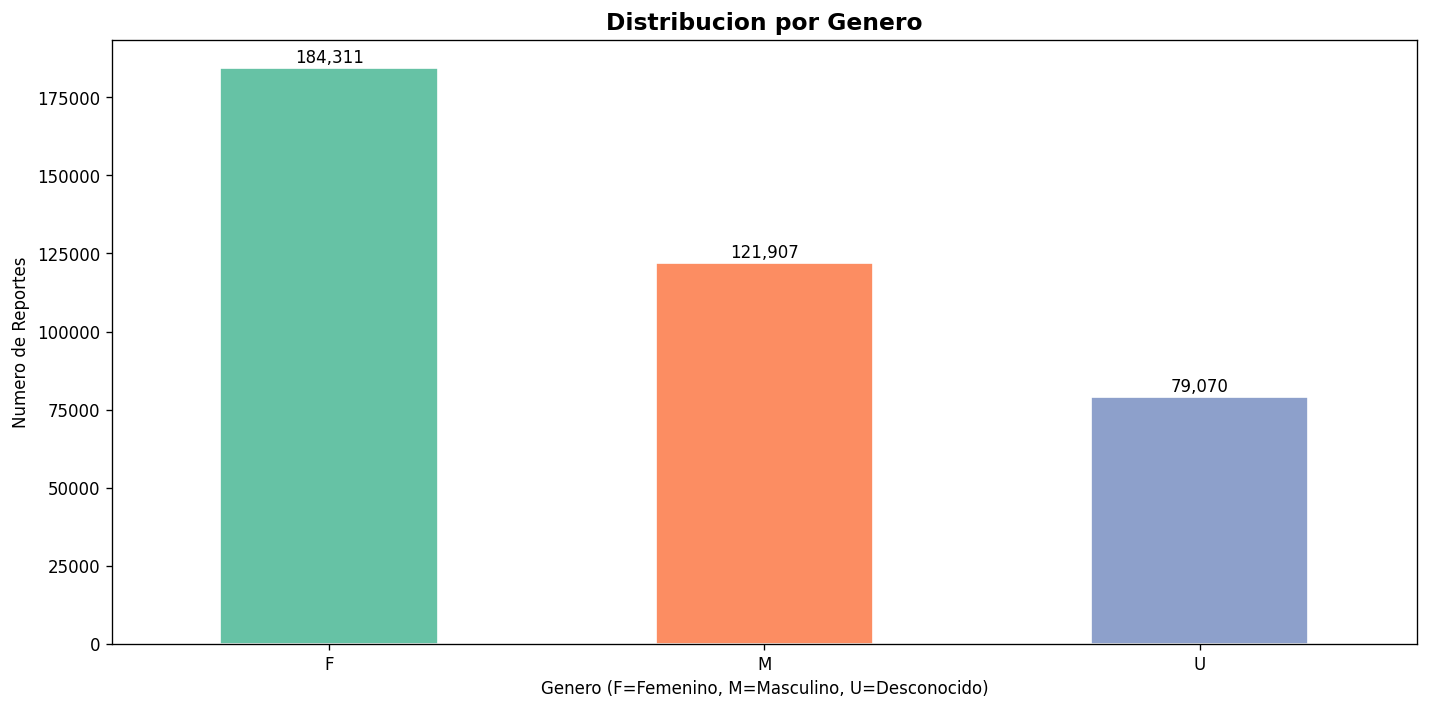
\includegraphics[width=0.70\textwidth]{eda_genero.png}
\caption{Distribución demográfica por sexo generada por el módulo EDA.}
\label{fig:eda}
\end{figure}

El EDA identificó miles de fármacos y términos MedDRA PT únicos, y reportes provenientes de más de 120 países con predominancia de Estados Unidos. En el componente demográfico, el sexo femenino fue el más frecuente, seguido del masculino y del desconocido. La edad media de los casos femeninos fue 54,3 años y la mediana 58 años, mientras que en los masculinos la media fue 53,9 años y la mediana 60 años. En medicamentos, DUPIXENT, ZEPBOUND y MOUNJARO aparecen entre los más reportados (Fig.~\ref{fig:eda_drug}). En reacciones adversas, destacan \textit{Off Label Use}, \textit{Drug Ineffective}, \textit{Product Dose Omission Issue}, fatiga, diarrea, náuseas y muerte.

\begin{figure}[H]
\centering
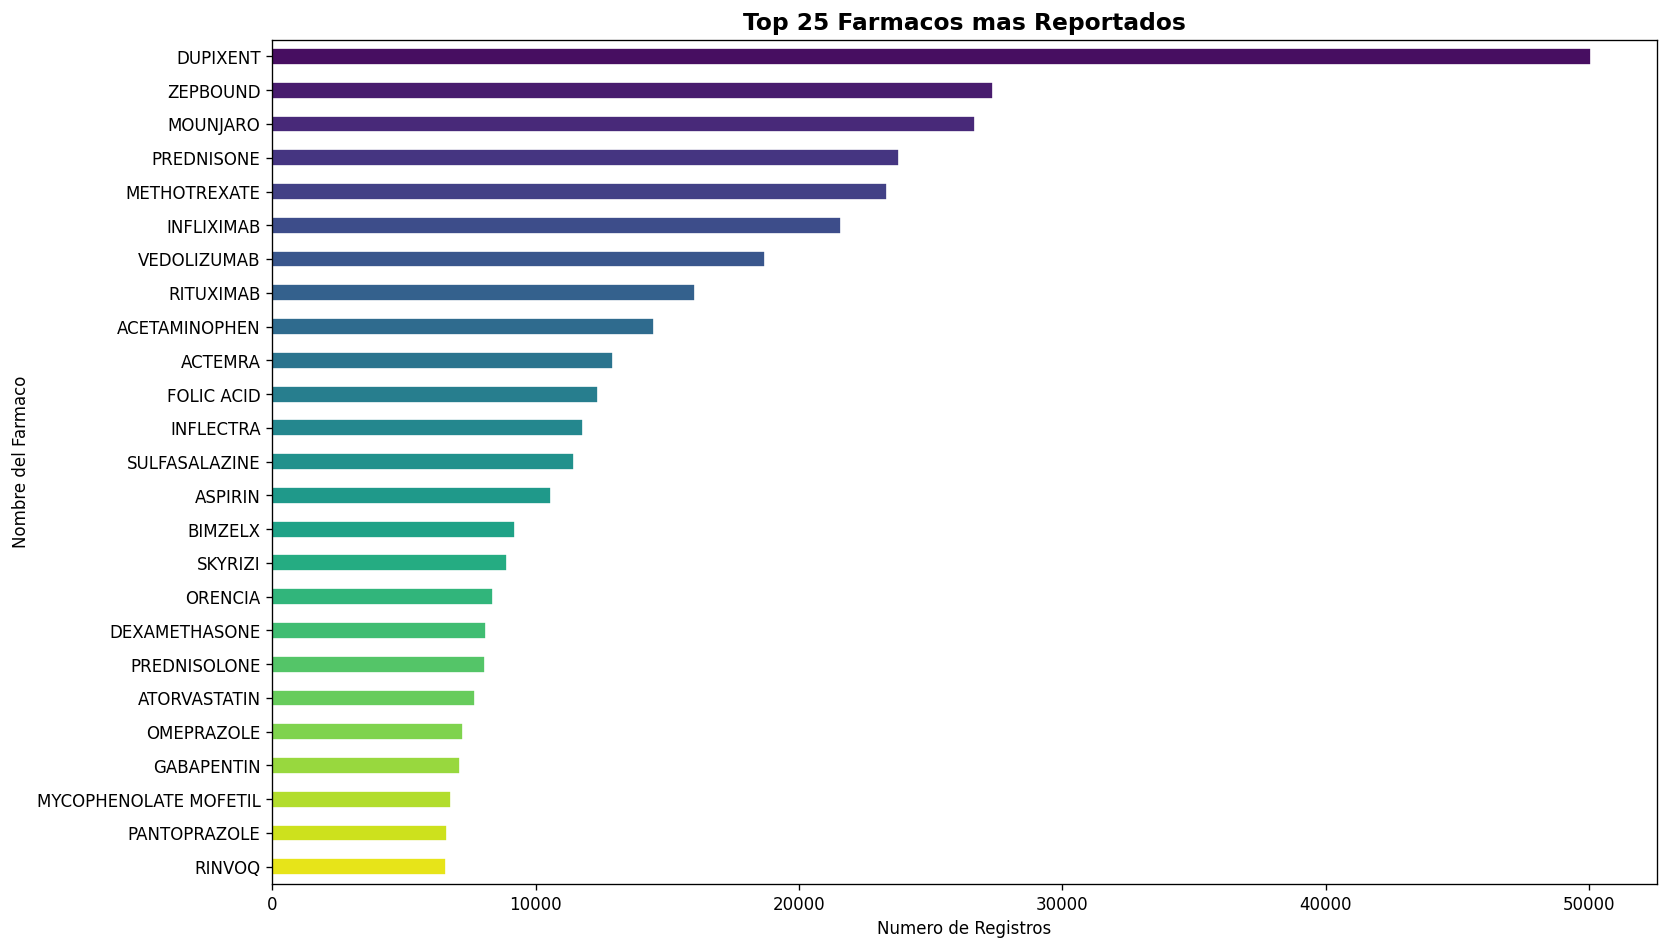
\includegraphics[width=0.86\textwidth]{eda_top_farmacos.png}
\caption{Medicamentos más reportados en el trimestre analizado.}
\label{fig:eda_drug}
\end{figure}

\subsection{Data Cleaning and Preprocessing}
La limpieza se desarrolló mediante scripts especializados por tabla (\texttt{s01} a \texttt{s07}, con consolidación en \texttt{s08}). Cada script realiza carga desde la capa \texttt{raw}, normalización de nombres de columnas, validaciones específicas, tratamiento de nulos, eliminación de duplicados y escritura del resultado en Parquet. El análisis de nulos guía decisiones automáticas: columnas con porcentajes muy altos de valores faltantes (por ejemplo, \texttt{exp\_dt}, \texttt{lot\_num} o \texttt{wt}) se descartan, mientras que campos con nulos moderados se imputan.

La normalización de \texttt{primaryid} fue crítica para resolver discrepancias de tipo entre tablas. Para ello, se eliminaron caracteres no numéricos y se convirtió el identificador a formato entero unificado. Esta operación redujo errores durante la unión distribuida y permitió aplicar un criterio de \textit{Inner Join} estricto.

\subsection{Feature Engineering and Leakage Control}
A partir del dataset consolidado se seleccionaron cuatro variables principales para el modelo predictivo: \texttt{drug\_encoded}, \texttt{pt\_encoded}, \texttt{sex\_encoded} y \texttt{age}. La Tabla~\ref{tab:features} presenta la transformación aplicada.

\begin{table}[H]
\centering
\caption{Características utilizadas para el entrenamiento predictivo.}
\label{tab:features}
\small
\begin{tabular}{@{}lll@{}}
\toprule
\textbf{Feature} & \textbf{Origen} & \textbf{Transformación} \\
\midrule
\texttt{drug\_encoded} & DRUG & \texttt{OrdinalEncoder} ajustado solo en \textit{train}. \\
\texttt{pt\_encoded} & REAC & \texttt{OrdinalEncoder} con enmascaramiento de \textit{proxies}. \\
\texttt{sex\_encoded} & DEMO & M=1,0; F=0,0; U=0,5 (dominio fijo). \\
\texttt{age} & DEMO & Conversión numérica e imputación (45,0). \\
\bottomrule
\end{tabular}
\end{table}

La variable objetivo \texttt{severity\_level} se derivó desde OUTC mediante el mapeo determinista implementado en el postprocesamiento del \textit{join}: el código \texttt{DE} (muerte) se asoció a nivel 5 (muy grave); \texttt{LT} (riesgo vital) a nivel 4 (grave); \texttt{HO} (hospitalización) y \texttt{CA} (anomalía congénita) a nivel 3 (importante); \texttt{DS} (discapacidad) y \texttt{RI} (intervención requerida) a nivel 2 (moderado); y \texttt{OT} (otro) a nivel 1 (leve). Cuando un caso presenta más de un desenlace, prevalece el de mayor severidad.

\paragraph{Escenario de despliegue y caso de uso operacional.} Dado que \texttt{severity\_level} se deriva determinísticamente de OUTC, es imprescindible precisar en qué momento del ciclo de vida del reporte se realiza la predicción; de lo contrario el problema sería trivial o circular. La tabla OUTC \textit{no} está disponible de forma inmediata ni completa al momento de ingreso de un reporte: en FAERS los reportes se reciben de manera incremental y con frecuencia incompleta, el desenlace puede notificarse en envíos posteriores (\textit{follow-up}) y, en reportes iniciales o de evolución abierta, el campo de desenlace puede estar ausente, ser provisional o llegar con retraso de semanas a meses respecto de la información de fármaco, reacción y demografía. El caso de uso del modelo es precisamente ese intervalo: \textit{estimar la severidad probable de un reporte entrante cuando DEMO, DRUG y REAC ya están presentes pero OUTC aún no se ha consolidado}, con el fin de priorizar la cola de revisión manual de farmacovigilancia (triaje) y disparar alertas tempranas sobre casos potencialmente graves antes del cierre del ciclo trimestral. En este escenario las \textit{features} (\texttt{drug}, \texttt{pt}, \texttt{sex}, \texttt{age}) provienen de tablas disponibles tempranamente, mientras que la etiqueta corresponde al desenlace que aún no se conoce; la predicción aporta valor justamente porque adelanta una estimación de la severidad final semanas antes de que OUTC esté disponible. Esta es también la razón por la cual el componente de \textit{streaming} (Sección~\ref{sec:streaming}) consume reportes ensamblados sin requerir un desenlace consolidado. Cuando OUTC sí está disponible, la etiqueta es conocida y el modelo no se utiliza para inferencia, sino únicamente como insumo de reentrenamiento.

El control de fuga de información se implementó en dos capas. En la primera capa, la partición \textit{train/test} (\texttt{test\_size=0.20}, \texttt{random\_state=42}, estratificada por clase) se ejecuta \textit{antes} de ajustar cualquier codificador y antes de aplicar SMOTE. Los codificadores ordinales de fármaco y reacción se ajustan (\texttt{fit}) exclusivamente sobre \(X_{\text{train}}\) y solo transforman \(X_{\text{test}}\); SMOTE se aplica posteriormente solo sobre el conjunto de entrenamiento, de modo que \(X_{\text{test}}\) e \(y_{\text{test}}\) permanecen intactos y libres de muestras sintéticas.

En la segunda capa se neutraliza el \textit{target leakage} de \texttt{pt\_encoded}. Para cada término MedDRA PT con al menos tres muestras en \(X_{\text{train}}\), se calcula la entropía de Shannon de su distribución de severidad:
\begin{equation}
H(\text{pt}) = -\sum_{k=1}^{5} p_k \log_2 p_k,
\end{equation}
donde \(p_k\) es la proporción de la clase de severidad \(k\) dentro del término. Los PT con \(H < 0{,}5\) revelan la etiqueta de forma casi determinista y se consideran \textit{proxies} del desenlace; estos términos se reemplazan por el centinela \texttt{OUTCOME\_PROXY}, preservando los términos legítimos. La lista de PT enmascarados se serializa (\texttt{leaking\_pt\_terms.json}) para reproducibilidad e inferencia. El procedimiento identificó 145 términos como \textit{proxies}, incluyendo \textit{Death}, \textit{Cardiac Arrest}, \textit{Hepatic Failure} y \textit{Multiple Organ Dysfunction Syndrome}.

El efecto del enmascaramiento se auditó mediante información mutua (\textit{mutual information}) entre cada \textit{feature} y \texttt{severity\_level}, calculada solo sobre \(X_{\text{train}}\). Se adoptó un umbral de 0,7 para señalar fuga: antes del enmascaramiento, \texttt{pt\_encoded} superaba dicho umbral, mientras que tras el enmascaramiento su información mutua quedó por debajo de 0,7, confirmando la neutralización de la señal determinista sin eliminar la información clínica legítima.

\subsection{Distributed MapReduce Join}
El \textit{Reduce-Side Join} fue implementado mediante \textit{mrjob}. En la etapa de preparación, cada tabla limpia se transforma a JSONL y cada registro se etiqueta con su tabla de origen. Luego, el \textit{mapper} emite pares de la forma \((primaryid, registro)\). El \textit{reducer} agrupa todos los registros asociados a un mismo \texttt{primaryid}, verifica la presencia de las tablas requeridas y emite un registro consolidado. Este diseño separa la lógica de negocio de la infraestructura de ejecución, de modo que la misma lógica de \textit{mapper} y \textit{reducer} puede ejecutarse localmente o en un clúster Hadoop real sin cambios sustanciales.

\subsection{Statistical Safety Signals}
Para cada par fármaco--reacción se calcularon métricas de desproporcionalidad. El PRR se definió como:

\begin{equation}
PRR = \frac{a/(a+b)}{c/(c+d)}
\end{equation}

donde \(a\) representa el número de reportes del fármaco con la reacción de interés, \(b\) el número de reportes del mismo fármaco con otras reacciones, \(c\) el número de reportes de otros fármacos con la reacción de interés y \(d\) los demás reportes. Adicionalmente, se aplicó Chi-cuadrado con corrección de Yates:

\begin{equation}
\chi^2 = \frac{N(|ad-bc|-N/2)^2}{(a+b)(c+d)(a+c)(b+d)}
\end{equation}

Se consideró señal relevante cuando un par cumplía tres condiciones: al menos tres reportes, \(PRR \geq 2.0\) y \(\chi^2 \geq 3.84\). Las señales detectadas se almacenaron en \texttt{top\_safety\_signals.csv} (más de 13.800 pares) e indexadas en memoria para consultas eficientes desde el consumidor Kafka.

\subsection{Class Balancing}
El desbalance de clases constituye uno de los principales desafíos del modelo de severidad. En el dataset consolidado utilizado para el balanceo, la clase mayoritaria (moderado) concentra cerca del 30,8\% de los casos y la clase muy grave alrededor del 3,7\%, con un ratio de desbalance aproximado de 8,3 veces. Se evaluaron varias familias de técnicas, resumidas en la Tabla~\ref{tab:balancing}, midiendo tamaño resultante y tiempo de ejecución.

\begin{table}[H]
\centering
\caption{Técnicas de balanceo evaluadas en el pipeline.}
\label{tab:balancing}
\small
\begin{tabular}{@{}llrr@{}}
\toprule
\textbf{Técnica} & \textbf{Familia} & \textbf{Filas resultado} & \textbf{Tiempo (s)} \\
\midrule
Random Undersampling & Undersampling & 15.038 & 0,4 \\
SMOTE & Oversampling & 313.470 & 15,4 \\
SMOTE-NC & Oversampling & 313.470 & 367,2 \\
SMOTE+ENN & Híbrida & 262.700 & 153,7 \\
\bottomrule
\end{tabular}
\end{table}

Para construir el conjunto de modelado se utilizó como entrada el \textit{dataset} balanceado por \textit{Random Undersampling} (15.038 registros), que iguala el soporte entre los cinco niveles de severidad y mantiene un tamaño manejable. Sobre esa base se aplicó además SMOTE como sobremuestreo, pero exclusivamente sobre el conjunto de entrenamiento y, durante la validación cruzada, encapsulado dentro de un \textit{pipeline}, de modo que cada pliegue de validación nunca observa muestras sintéticas. La etapa de preparación selecciona dinámicamente el \textit{dataset} balanceado disponible, por lo que la técnica de balanceo de base es configurable sin alterar el resto del flujo.

\subsection{Predictive Modeling and Model Comparison}
A diferencia de la versión previa, basada en un clasificador único, esta etapa compara cuatro modelos: una Regresión Logística como línea base, un Random Forest (100 árboles, profundidad máxima 16, \texttt{class\_weight='balanced'}), XGBoost y LightGBM. Todos utilizan semilla fija 42.

El protocolo de evaluación encadena SMOTE y el clasificador dentro de un \textit{pipeline} de \texttt{imbalanced-learn} (\texttt{ImbPipeline}), que se valida mediante \texttt{StratifiedKFold} de cinco pliegues con \(F_1\) macro como métrica. De esta forma, SMOTE se ajusta solo sobre el pliegue de entrenamiento de cada iteración, evitando contaminar el pliegue de validación. La partición estratificada (80/20) produjo 12.030 registros de entrenamiento y 3.008 de prueba. Para el entrenamiento final, cada modelo se ajusta sobre el conjunto de entrenamiento remuestreado con SMOTE y se evalúa sobre el conjunto de prueba intacto. Las etiquetas se desplazan de \([1,5]\) a \([0,4]\) por compatibilidad con XGBoost. El mejor modelo, según \(F_1\) macro en prueba, se serializa con \textit{joblib} junto con los codificadores.

\subsection{Streaming Architecture}
\label{sec:streaming}
El componente streaming se implementó mediante un productor y consumidor Kafka. El productor ensambla reportes por \texttt{primaryid} desde la capa cruda FAERS. El consumidor evalúa cada evento entrante, consulta señales históricas indexadas por par fármaco--reacción y aplica el modelo entrenado para estimar severidad, generando alertas cuando la predicción indica severidad grave (4) o muy grave (5). En caso de no existir un broker Kafka disponible, el sistema utiliza una cola local implementada con \texttt{queue.Queue}, manteniendo continuidad operativa en pruebas locales y registrando diagnósticos en \texttt{logs/streaming\_pipeline.log}.

\section{Results}

\subsection{Dataset Characterization}
El dataset procesado contiene 5.473.692 registros y 385.288 casos únicos. Los registros se distribuyen en siete tablas, siendo DRUG, REAC e INDI las de mayor volumen. La caracterización inicial reveló miles de fármacos y términos MedDRA PT únicos y más de 120 países reportantes, con predominancia de Estados Unidos. En medicamentos, DUPIXENT, ZEPBOUND y MOUNJARO aparecen entre los más reportados. En reacciones adversas, destacan \textit{Off Label Use}, \textit{Drug Ineffective}, \textit{Product Dose Omission Issue}, fatiga, diarrea, náuseas y muerte.

\subsection{Clinical Outcome Distribution}
La Tabla~\ref{tab:outc} presenta la distribución de desenlaces clínicos OUTC. El código OT concentra 55,7\% de los registros, seguido por hospitalización (27,8\%) y muerte (9,1\%).

\begin{table}[H]
\centering
\caption{Distribución de desenlaces clínicos OUTC.}
\label{tab:outc}
\small
\begin{tabular}{@{}llrr@{}}
\toprule
\textbf{Código} & \textbf{Descripción} & \textbf{Conteo} & \textbf{\%} \\
\midrule
OT & Otro resultado & 161.458 & 55,7 \\
HO & Hospitalización & 80.556 & 27,8 \\
DE & Muerte & 26.291 & 9,1 \\
LT & Riesgo vital & 13.126 & 4,5 \\
DS & Discapacidad & 6.065 & 2,1 \\
CA & Anomalía congénita & 1.371 & 0,5 \\
RI & Intervención requerida & 854 & 0,3 \\
\bottomrule
\end{tabular}
\end{table}

\begin{figure}[H]
\centering
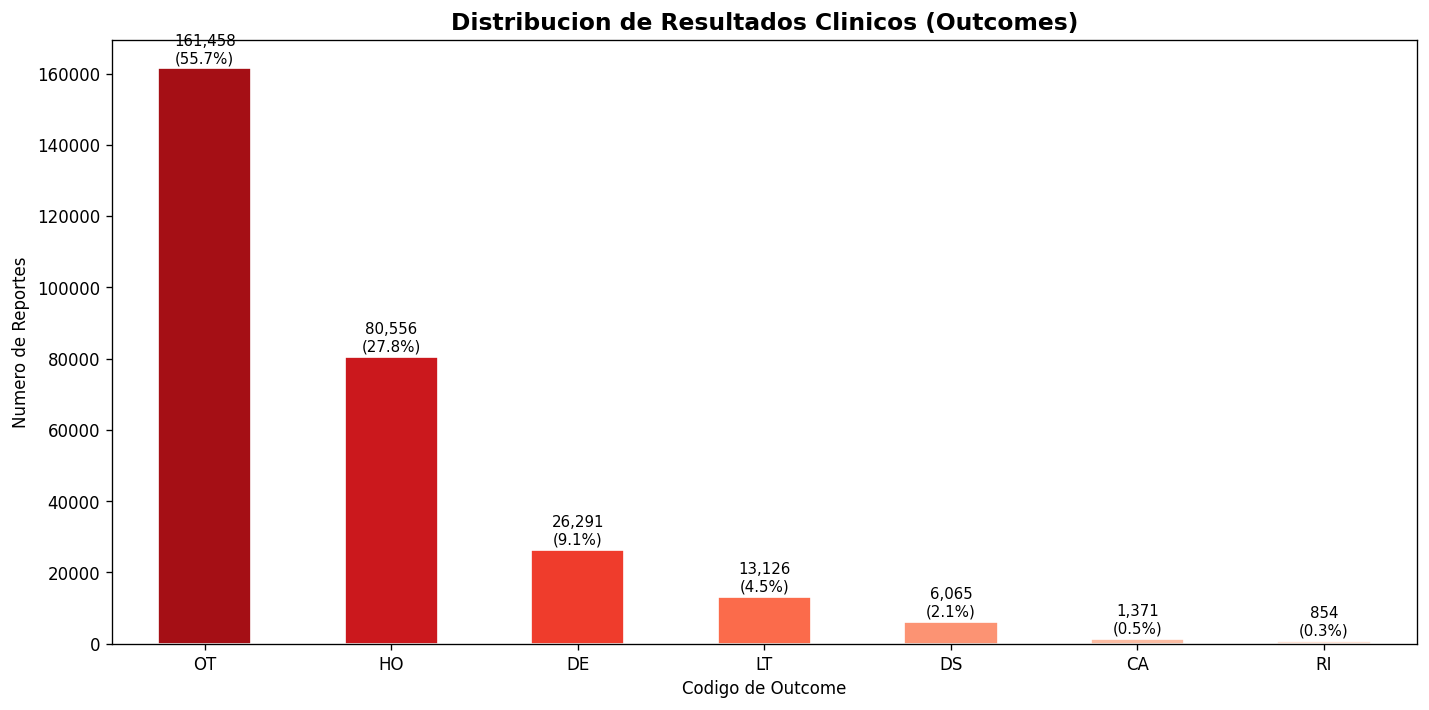
\includegraphics[width=0.78\textwidth]{eda_outcomes.png}
\caption{Distribución de desenlaces clínicos en la tabla OUTC.}
\label{fig:eda_outc}
\end{figure}

\subsection{Exploratory Analysis Results}
El EDA confirmó una estructura fuertemente desbalanceada en severidad clínica, consistente con la concentración de desenlaces leves y moderados. Esta distribución justifica el uso de estrategias de balanceo y de métricas por clase, ya que la exactitud global puede ser engañosa en escenarios clínicos desbalanceados. La matriz de co-ocurrencia fármaco--reacción mostró asociaciones frecuentes que luego sirvieron como base para el cálculo de señales estadísticas.

\subsection{Cleaning and Storage Results}
El proceso de limpieza generó archivos Parquet para cada tabla FAERS. La conversión a formato columnar redujo el tamaño respecto de los archivos de texto plano y aceleró la lectura en etapas posteriores. El uso de logs de auditoría permitió registrar filas iniciales, filas eliminadas, valores imputados y resultados finales por tabla, así como las decisiones automáticas de descarte o imputación de columnas según su porcentaje de nulos.

\subsection{Distributed Join Results}
La preparación de entradas para MapReduce produjo archivos JSONL etiquetados por tabla. Posteriormente, el \textit{Reduce-Side Join} consolidó los registros por \texttt{primaryid}, generando el dataset analítico empleado en los módulos de señales y modelado. El enfoque demostró ser adecuado para separar la lógica de negocio de la infraestructura de ejecución.

\subsection{Safety Signal Results}
El módulo de señales generó más de 13.800 pares fármaco--reacción que cumplen simultáneamente los criterios de soporte mínimo, \(PRR \geq 2.0\) y \(\chi^2 \geq 3.84\). Entre los pares con mayor \(\chi^2\) aparecen asociaciones plausibles desde el punto de vista clínico, como factores de coagulación con eventos hemorrágicos. Estos resultados deben interpretarse como indicios de desproporcionalidad para revisión experta, no como evidencia causal.

\subsection{Leakage-Control Results}
La auditoría de información mutua sobre \(X_{\text{train}}\) confirmó la efectividad del control de fuga. Tras enmascarar los 145 términos MedDRA identificados como \textit{proxies}, la información mutua de \texttt{pt\_encoded} respecto de \texttt{severity\_level} descendió por debajo del umbral de fuga (0,7), preservando los términos clínicamente informativos. Esta corrección es la principal responsable de que las métricas de desempeño reportadas sean realistas y no estén infladas por variables que codifican el desenlace.

\subsection{Predictive Evaluation}
La Tabla~\ref{tab:model_comparison} resume la comparación de los cuatro modelos. La validación cruzada de cinco pliegues (Fig.~\ref{fig:cv}) muestra que los modelos basados en árboles superan ampliamente la línea base lineal y exhiben un desempeño muy estable entre pliegues. Sobre el conjunto de prueba intacto, Random Forest obtuvo el mayor \(F_1\) macro (0,517) y la mayor exactitud (0,689), seguido muy de cerca por XGBoost y LightGBM, mientras que la Regresión Logística quedó claramente rezagada.

\begin{table}[H]
\centering
\caption{Comparación de modelos: validación cruzada y desempeño en el conjunto de prueba intacto.}
\label{tab:model_comparison}
\small
\begin{tabular}{@{}lrrrr@{}}
\toprule
\textbf{Modelo} & \textbf{CV \(F_1\) (media)} & \textbf{CV \(F_1\) (desv.)} & \textbf{Test \(F_1\) macro} & \textbf{Test Acc.} \\
\midrule
Baseline (LR) & 0,295 & 0,014 & 0,284 & 0,441 \\
Random Forest & 0,502 & 0,008 & \textbf{0,517} & \textbf{0,689} \\
XGBoost & 0,503 & 0,011 & 0,514 & 0,683 \\
LightGBM & 0,505 & 0,013 & 0,504 & 0,678 \\
\bottomrule
\end{tabular}
\end{table}

\begin{figure}[H]
\centering
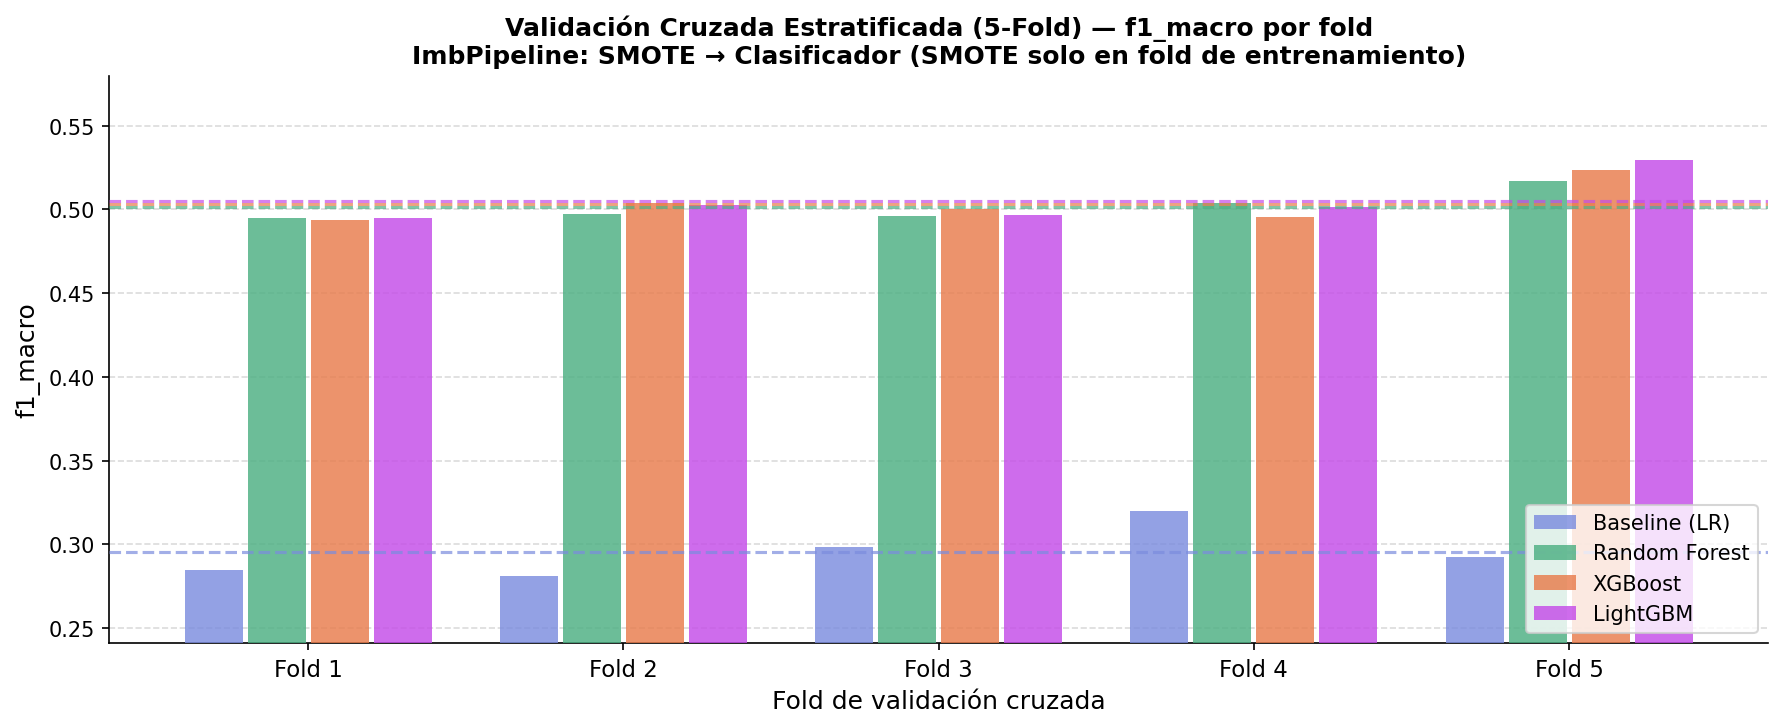
\includegraphics[width=0.92\textwidth]{cv_fold_scores.png}
\caption{Validación cruzada estratificada de cinco pliegues (\(F_1\) macro por pliegue). SMOTE se aplica solo en el pliegue de entrenamiento dentro del \textit{pipeline}.}
\label{fig:cv}
\end{figure}

El análisis por clase del modelo seleccionado (Random Forest) muestra un desempeño muy alto en la clase muy grave (nivel 5: precisión 0,928, \textit{recall} 0,961, \(F_1\) 0,944), favorecida por su gran soporte en el conjunto de prueba, y un desempeño más modesto en las clases intermedias, especialmente el nivel 4 (grave), que resulta el más difícil de separar. Las matrices de confusión de los cuatro modelos (Fig.~\ref{fig:cm}) y las curvas ROC One-vs-Rest con promedio macro (Fig.~\ref{fig:roc}) confirman este patrón: Random Forest alcanza un AUC macro de 0,867, seguido por LightGBM (0,861) y XGBoost (0,852), muy por encima de la línea base (0,646).

\begin{figure}[H]
\centering
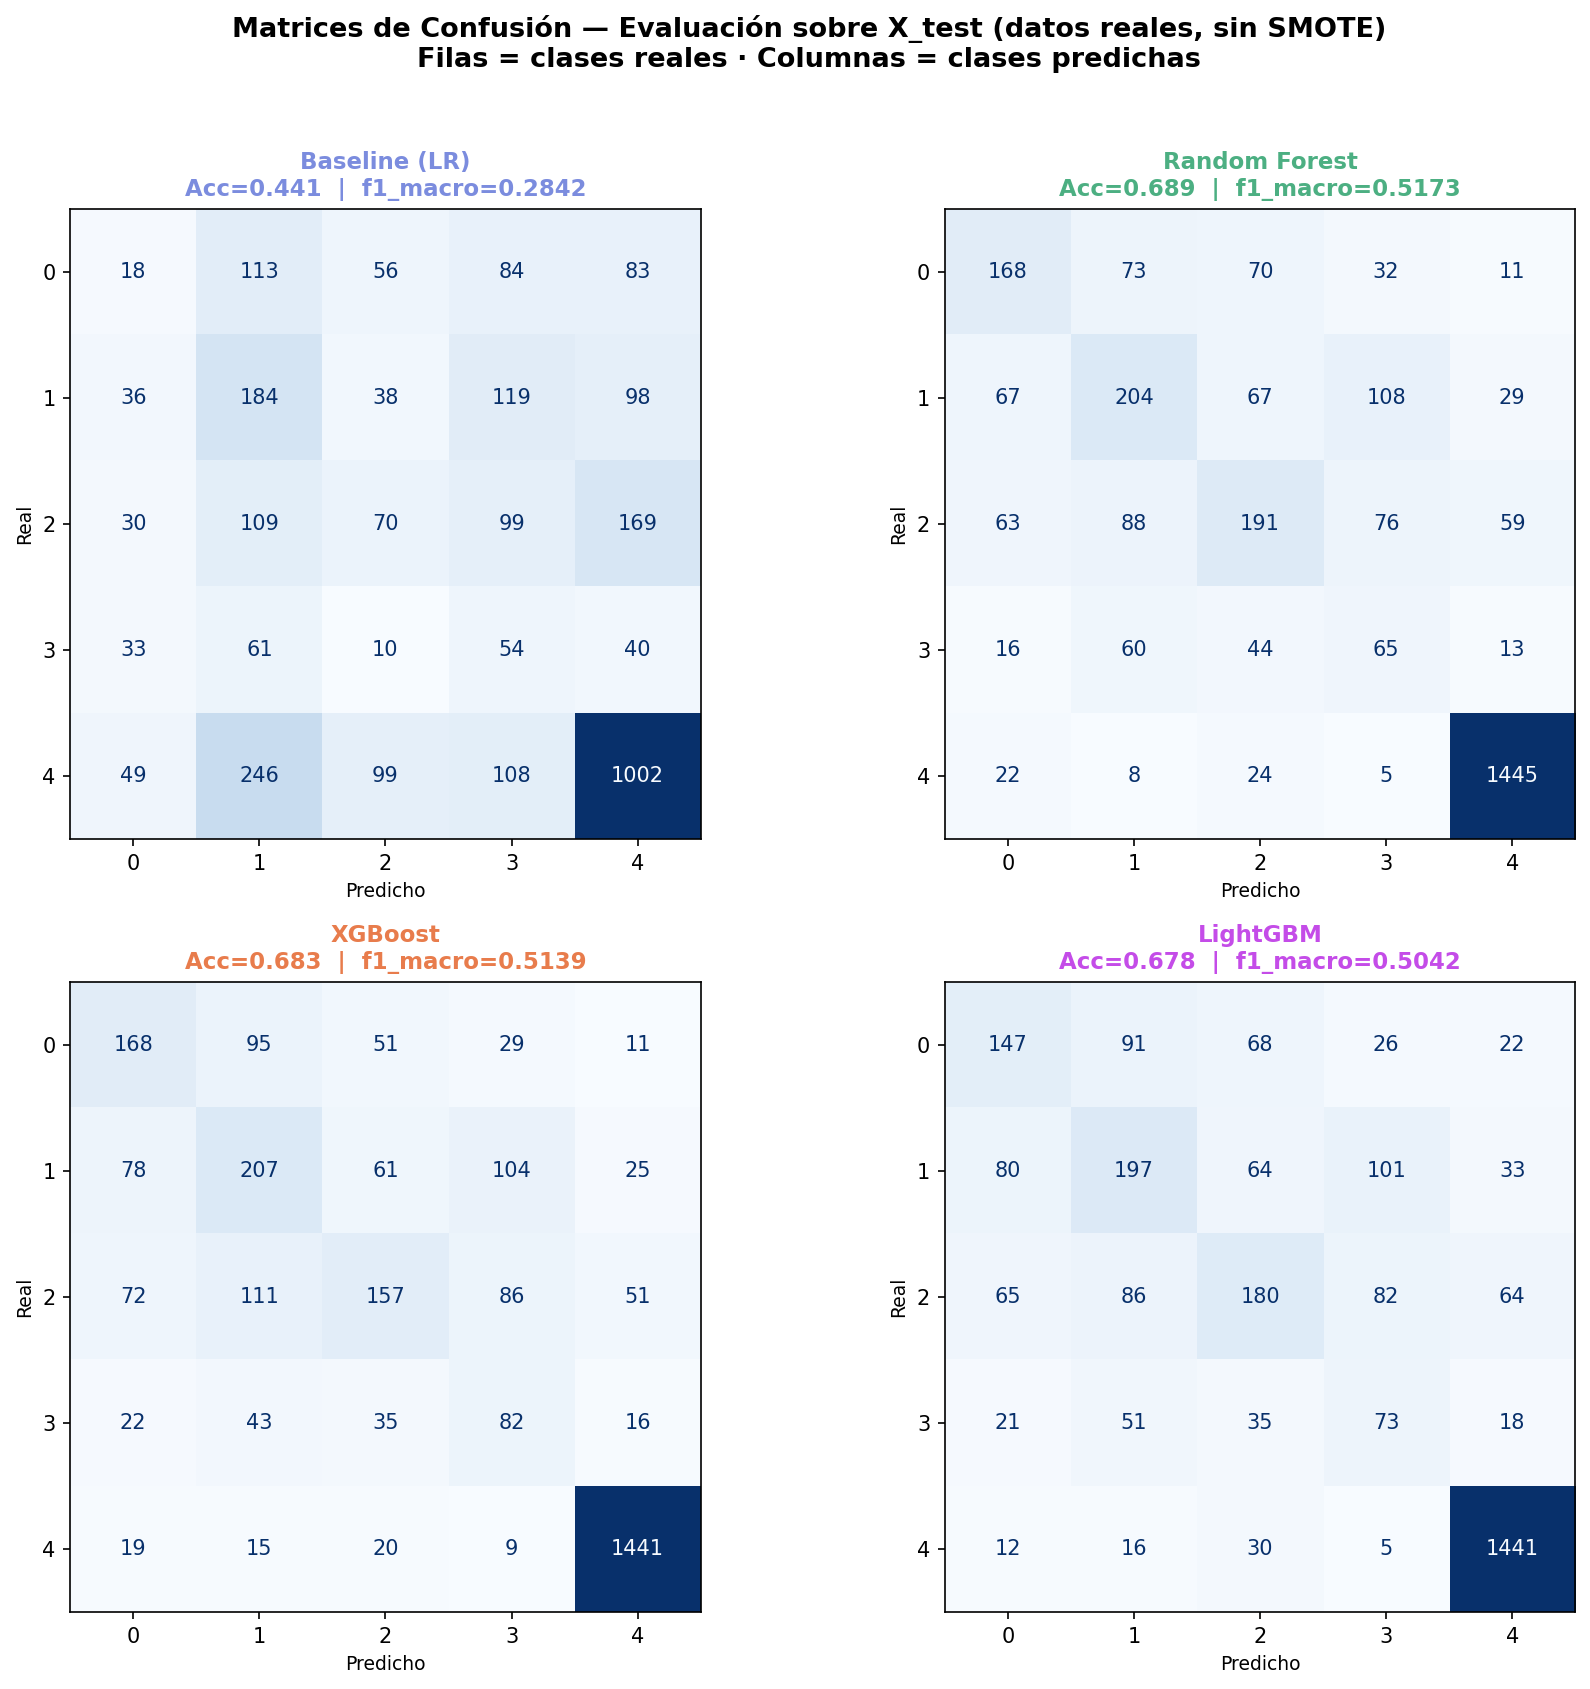
\includegraphics[width=0.92\textwidth]{confusion_matrices.png}
\caption{Matrices de confusión de los cuatro modelos evaluadas sobre el conjunto de prueba real (sin muestras sintéticas). Filas: clases reales; columnas: clases predichas.}
\label{fig:cm}
\end{figure}

\begin{figure}[H]
\centering
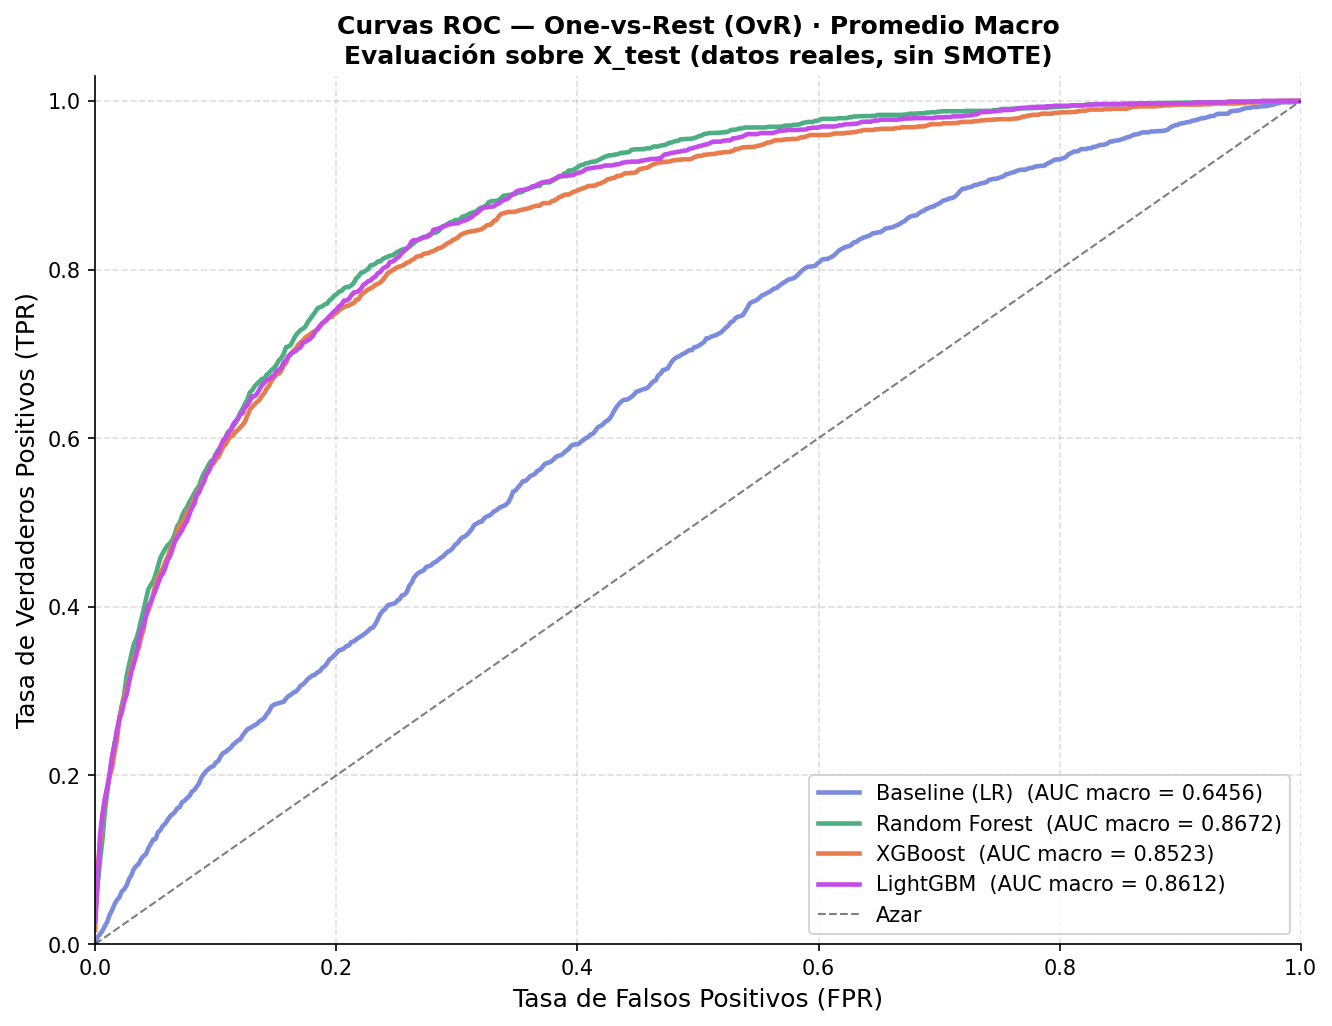
\includegraphics[width=0.80\textwidth]{roc_curves.png}
\caption{Curvas ROC One-vs-Rest con promedio macro por modelo, evaluadas sobre el conjunto de prueba real.}
\label{fig:roc}
\end{figure}

Los resultados muestran que el modelo reconoce patrones asociados a severidad a partir de variables de medicamento, reacción, sexo y edad. A diferencia de evaluaciones previas, estas métricas se obtienen sobre datos reales sin contaminación sintética y sin variables que codifiquen el desenlace, por lo que constituyen una estimación honesta del desempeño. Su interpretación debe realizarse con cautela, ya que FAERS no representa incidencia poblacional y las clases críticas pueden estar condicionadas por subregistro o sesgos de reporte.

\subsection{Streaming Validation}
El componente de streaming permitió simular la evaluación de reportes entrantes y generar alertas cuando se detectaban combinaciones fármaco--reacción relevantes o severidades altas. La validación confirmó que el sistema opera en dos modos: con broker Kafka real o con cola local simulada. Esta dualidad mejora la portabilidad y permite ejecutar demostraciones del pipeline sin requerir un despliegue completo de infraestructura distribuida.

\section{Discussion}

\subsection{Technical Contributions}
La principal contribución técnica de este trabajo es la integración coherente de tecnologías Big Data, estadística de farmacovigilancia y aprendizaje automático dentro de un único pipeline reproducible y, en esta versión, metodológicamente riguroso frente a la fuga de información. El sistema no se limita a ejecutar un modelo aislado: incluye ingestión, limpieza, almacenamiento por capas, unión distribuida, cálculo de señales, balanceo, comparación de modelos con validación cruzada e inferencia en tiempo real. El control de fuga en dos capas y la comparación sistemática de cuatro algoritmos diferencian este trabajo de su versión anterior y elevan la credibilidad de las métricas reportadas.

\subsection{Clinical and Operational Implications}
Desde una perspectiva clínica, el sistema permite priorizar combinaciones fármaco--reacción que cumplen criterios estadísticos de señal, apoyando procesos de revisión experta y monitoreo de medicamentos con patrones inusuales. No obstante, las señales deben entenderse como indicios para análisis posterior, no como evidencia causal definitiva. Desde una perspectiva operacional, el valor del componente predictivo no está en reproducir un desenlace ya registrado, sino en anticiparlo: cuando un reporte ingresa con información de fármaco, reacción y demografía pero sin un desenlace OUTC consolidado, el modelo entrega una estimación temprana de severidad que permite ordenar la cola de revisión manual (triaje) y elevar casos potencialmente graves para evaluación prioritaria, semanas antes del cierre del ciclo trimestral. Kafka materializa esta capacidad al evaluar reportes nuevos sin esperar el lote completo. Las métricas moderadas pero honestas reportadas deben leerse a la luz de este caso de uso: incluso una clasificación gruesa en niveles de severidad es operacionalmente útil para triaje, donde el costo de revisar un caso es bajo frente al costo de omitir un evento grave.

\subsection{Limitations}
El estudio presenta varias limitaciones. Primero, FAERS es un sistema de reporte espontáneo; por tanto, los datos están sujetos a subregistro, duplicación, sesgos de notificación y ausencia de denominadores poblacionales, y nuestro pipeline no realiza el mapeo completo a vocabularios estándar (RxNorm, SNOMED-CT) que recursos curados como AEOLUS~\cite{banda2016} sí aplican. Segundo, una asociación fármaco--reacción frecuente no implica causalidad. Tercero, el uso de codificación ordinal para variables de alta cardinalidad (fármaco y reacción) impone un orden numérico artificial entre categorías que no tienen relación de orden intrínseca; aunque los modelos basados en árboles son relativamente robustos a esta codificación, representaciones como \textit{embeddings} categóricos o \textit{target encoding} con validación anidada serían preferibles y se dejan como trabajo futuro. Cuarto, el enmascaramiento de \textit{proxies} basado en entropía, si bien neutraliza la fuga, también reduce el techo de desempeño alcanzable, lo que explica métricas más moderadas pero honestas. Quinto, el modelo se entrena y evalúa sobre un único trimestre (2025\,Q4) con partición aleatoria estratificada; no se realiza validación temporal (entrenar en trimestres anteriores y evaluar en posteriores), por lo que la estabilidad de las señales y del modelo ante la deriva temporal queda sin demostrar empíricamente. Sexto, el componente de \textit{streaming} con Kafka es, en su forma actual, una demostración funcional: se valida principalmente sobre una cola local (\texttt{queue.Queue}) y no constituye un despliegue productivo con un \textit{broker} distribuido bajo carga real, garantías de entrega o tolerancia a fallos. Estas limitaciones acotan el alcance de las conclusiones y orientan directamente las líneas de trabajo futuro.

\subsection{Reproducibility}
El pipeline fue diseñado para ser reproducible mediante scripts numerados, rutas estandarizadas y artefactos intermedios. El uso de semilla fija 42 en partición, balanceo y entrenamiento contribuye a estabilizar resultados. La serialización de modelos y codificadores mediante \textit{joblib}, junto con la lista de términos enmascarados (\texttt{leaking\_pt\_terms.json}) y la tabla comparativa (\texttt{model\_comparison.json}), permite reutilizar y auditar los activos entrenados en inferencia posterior. Para que la reproducibilidad sea efectiva y no solo declarativa, el repositorio asociado~\cite{repoFaers} se publica con acceso abierto e incluye: un \texttt{README} con instrucciones de ejecución paso a paso, un archivo de dependencias con versiones fijadas (\texttt{requirements.txt}), un subconjunto de datos de ejemplo que permite ejecutar el flujo completo sin descargar el trimestre íntegro, los scripts de las etapas \texttt{s01}--\texttt{s09} y los artefactos serializados mencionados (modelos, codificadores, \texttt{leaking\_pt\_terms.json} y \texttt{model\_comparison.json}). Dado que los datos FAERS originales son de dominio público, el repositorio documenta además el procedimiento exacto de descarga y la versión trimestral empleada (2025\,Q4), de modo que un tercero pueda regenerar todos los resultados reportados.

\section{Future Work}
\label{sec:future}
Futuras líneas de trabajo incluyen extender el análisis a múltiples trimestres FAERS para evaluar la estabilidad temporal de señales y del modelo predictivo, así como migrar la ejecución desde modo local hacia un clúster Hadoop o un motor Spark real, manteniendo sin cambios la lógica principal del \textit{mapper} y \textit{reducer}. Esta extensión multitrimestral es además la vía para justificar empíricamente la infraestructura distribuida: al acumular el histórico de FAERS (decenas de trimestres, cientos de millones de registros) el volumen agregado superará la capacidad de un solo nodo y permitirá medir el escalamiento real (\textit{strong} y \textit{weak scaling}) de la unión distribuida, complementando la validación de portabilidad realizada en este trabajo a escala de un trimestre. En esa misma línea, se prevé incorporar validación temporal estricta (entrenar en trimestres tempranos y evaluar en posteriores) para cuantificar la deriva del modelo, y consolidar el componente de \textit{streaming} desde su forma actual de demostración hacia un despliegue con \textit{broker} Kafka distribuido y garantías de entrega.

Desde el modelado, se propone incorporar embeddings categóricos para representar medicamentos y reacciones sin imponer relaciones ordinales artificiales, explorar calibración de probabilidades y métricas sensibles al costo clínico, y profundizar en la clase grave (nivel 4), que resultó la más difícil de separar. Desde la perspectiva de farmacovigilancia, el trabajo futuro debería incluir validación clínica de señales detectadas, comparación con bases externas como OpenFDA o literatura biomédica, y evaluación longitudinal de señales emergentes a través de trimestres sucesivos.

\section{Conclusions}
Este trabajo presentó una arquitectura distribuida para análisis predictivo de farmacovigilancia sobre reportes FAERS, con énfasis en la honestidad metodológica. El sistema procesó 5.473.692 registros correspondientes a 385.288 casos únicos, integrando limpieza, almacenamiento columnar, análisis exploratorio, \textit{Reduce-Side Join}, señales PRR/Chi-cuadrado, balanceo de clases, comparación de modelos y streaming con Kafka.

La incorporación de un control de fuga de información en dos capas —partición previa al ajuste de transformaciones y enmascaramiento por entropía de \textit{proxies} de desenlace— permitió obtener métricas realistas: el mejor modelo (Random Forest) alcanzó una exactitud de 0,689, un \(F_1\) macro de 0,517 y un AUC macro de 0,867 sobre datos reales, superando a XGBoost, LightGBM y a una línea base lineal. Los resultados demuestran que una arquitectura híbrida batch--streaming puede mejorar la escalabilidad y oportunidad del análisis de eventos adversos, mientras que un protocolo de modelado riguroso evita conclusiones infladas.

La propuesta constituye una base técnica extensible para sistemas de vigilancia farmacológica más robustos, reproducibles y preparados para el crecimiento continuo de datos clínicos. Si bien los resultados no deben interpretarse como causalidad clínica, el sistema entrega una herramienta útil para priorización, análisis exploratorio y apoyo a la revisión experta.

\section*{Acknowledgements}
Los autores agradecen a la Universidad Andrés Bello y a la asignatura Ciencia de Datos por el marco académico para el desarrollo del proyecto. Este trabajo fue realizado en el contexto de formación en Ingeniería Civil Informática.

\section*{References}

\begin{thebibliography}{99}

\bibitem{faers2025}
U.S. Food and Drug Administration. \textit{FDA Adverse Event Reporting System (FAERS)}. 2025. \url{https://www.fda.gov/drugs/surveillance/fda-adverse-event-reporting-system-faers}

\bibitem{banda2016}
Banda, J. M., Evans, L., Vanguri, R. S., Tatonetti, N. P., Ryan, P. B., \& Shah, N. H. (2016). A curated and standardized adverse drug event resource to accelerate drug safety research. \textit{Scientific Data}, 3, 160026.

\bibitem{evans2001}
Evans, S. J. W., Waller, P. C., \& Davis, S. (2001). Use of proportional reporting ratios (PRRs) for signal generation from spontaneous adverse drug reaction reports. \textit{Pharmacoepidemiology and Drug Safety}, 10(6), 483--486.

\bibitem{ema2006}
European Medicines Agency. (2006). \textit{Guideline on the use of statistical signal detection methods in the EudraVigilance data analysis system}. EMEA/106464/2006.

\bibitem{disproportionalityAssessment2015}
Disproportionality measures used in signal detection: an assessment on pharmacovigilance adverse event reporting system data. (2015). \textit{Value in Health}, 18(7), A719.

\bibitem{ticagrelorFaers2024}
A disproportionality analysis of FDA Adverse Event Reporting System (FAERS) events for ticagrelor. (2024). \textit{Frontiers in Pharmacology}, 15, 1251961.

\bibitem{il1faers2024}
Disproportionality analysis of adverse events associated with IL-1 inhibitors in the FDA Adverse Event Reporting System (FAERS). (2024). \textit{Pharmaceuticals}.

\bibitem{nguyenSurvey2021}
Nguyen, D. A., Nguyen, C. H., \& Mamitsuka, H. (2021). A survey on adverse drug reaction studies: data, tasks and machine learning methods. \textit{Briefings in Bioinformatics}, 22(1), 164--177.

\bibitem{oncoSAE2026}
Machine learning model for predicting severe adverse events in oncology patients using the US FDA Adverse Event Reporting System. (2026). \textit{JCO Clinical Cancer Informatics}.

\bibitem{pd1faers2025}
Machine learning-based prediction of adverse events in cancer patients treated with PD-1/PD-L1 inhibitors using FAERS data. (2025).

\bibitem{automatingADE2024}
Automating adverse event detection in clinical trials through machine learning. (2024).

\bibitem{ensembleRare2026}
Early detection of signals in pharmacovigilance: a machine learning ensemble approach to identify rare adverse drug reactions. (2026). \textit{medRxiv} preprint.

\bibitem{kaufman2012}
Kaufman, S., Rosset, S., Perlich, C., \& Stitelman, O. (2012). Leakage in data mining: formulation, detection, and avoidance. \textit{ACM Transactions on Knowledge Discovery from Data}, 6(4), 1--21.

\bibitem{chawla2002}
Chawla, N. V., Bowyer, K. W., Hall, L. O., \& Kegelmeyer, W. P. (2002). SMOTE: Synthetic Minority Over-sampling Technique. \textit{Journal of Artificial Intelligence Research}, 16, 321--357.

\bibitem{lemaitre2017}
Lema\^itre, G., Nogueira, F., \& Aridas, C. K. (2017). Imbalanced-learn: a Python toolbox to tackle the curse of imbalanced datasets in machine learning. \textit{Journal of Machine Learning Research}, 18(17), 1--5.

\bibitem{chen2016}
Chen, T., \& Guestrin, C. (2016). XGBoost: a scalable tree boosting system. \textit{Proc. 22nd ACM SIGKDD Int. Conf. on Knowledge Discovery and Data Mining}, 785--794.

\bibitem{ke2017}
Ke, G., Meng, Q., Finley, T., Wang, T., Chen, W., Ma, W., Ye, Q., \& Liu, T.-Y. (2017). LightGBM: a highly efficient gradient boosting decision tree. \textit{Advances in Neural Information Processing Systems}, 30, 3146--3154.

\bibitem{pedregosa2011}
Pedregosa, F. et al. (2011). Scikit-learn: machine learning in Python. \textit{Journal of Machine Learning Research}, 12, 2825--2830.

\bibitem{hadoop}
Apache Software Foundation. \textit{Apache Hadoop MapReduce Framework Documentation}. \url{https://hadoop.apache.org/docs/current/}

\bibitem{spark}
Zaharia, M. et al. (2016). Apache Spark: a unified engine for big data processing. \textit{Communications of the ACM}, 59(11), 56--65.

\bibitem{mrjob}
Yelp Inc. \textit{mrjob: MapReduce on Python}. \url{https://mrjob.readthedocs.io/}

\bibitem{kafka}
Apache Software Foundation. \textit{Apache Kafka Documentation}. \url{https://kafka.apache.org/documentation/}

\bibitem{arrow}
Apache Software Foundation. \textit{Apache Arrow and PyArrow Documentation}. \url{https://arrow.apache.org/docs/python/}

\bibitem{repoFaers}
Barrientos, N. et al. \textit{Proyecto Big Data FAERS}. GitHub repository. \url{https://github.com/Nico8270/Proyecto-Big-Data-FAERS}

\bibitem{ANAMED2026}
Instituto de Salud Pública de Chile. (2026). \textit{Agencia Nacional de Medicamentos (ANAMED)}. \url{https://www.ispch.gob.cl/anamed/}

\end{thebibliography}
\end{document}
